\documentclass[11pt]{article}
\usepackage[utf8]{inputenc}
\usepackage[english]{babel}
\usepackage{amsmath}
\usepackage{graphicx}
\usepackage{float}
\usepackage{lipsum}
\usepackage{multicol}
\usepackage{xcolor}
\usepackage{tabularx}
\usepackage{booktabs}
\usepackage{hyperref}
\usepackage{enumitem}
\newcolumntype{Y}{>{\centering\arraybackslash}X}
\usepackage[left=2.00cm, right=2.00cm, top=2.00cm, bottom=2.00cm]{geometry}

\title{AN2DL Reports Template}

\begin{document}
    
    \begin{figure}[H]
        \raggedright
        
\includegraphics[scale=0.5]{polimi} \hfill 
\includegraphics[scale=0.3]{airlab}
    \end{figure}
    \vspace{5mm}

    \begin{center}
        % Select between First and Second
        {\Large \textbf{AN2DL - First Challenge Report}}\\
        \vspace{2mm}
        % Change with your Team Name
        {\Large \textbf{I Neuroni Ribelli}}\\
        \vspace{2mm}
        % Team Members Information
        {\large Alberto Ondei,}
        {\large Andrea Valentini,}
        {\large Abdullah Javed,}
        {\large Filippo Barbari}\\
        \vspace{2mm}
        % Codabench Nicknames
        {albertoondei,}
        {andrevale69,}
        {javedhercules,}
        {filippobarbari}\\
        \vspace{2mm}
        % Matriculation Numbers
        {??????,}
        {??????,}
        {??????,}
        {??????}\\
        \vspace{5mm}
        \today
    \end{center}
    \vspace{5mm}
    
    \begin{multicols}{2}
        \section{Introduction}

        The goal of this challenge was to predict the \textbf{true pain level} of each subject from multivariate time–series data.
        Our work focused on three main objectives:
        \begin{itemize}[nosep]
            \item \textbf{Identify} the roles of static features vs dynamic joint signals;
            \item \textbf{Model} temporal patterns effectively, avoiding overfitting;
            \item \textbf{Address} the strong imbalance between the three pain classes.
        \end{itemize}
        We adopted a step-by-step approach:
        \begin{enumerate}[nosep]
            \item Initial EDA and establishment of a \textbf{baseline model} separating static and dynamic inputs (in Notebook 1);
            \item Notebook 2 focuses on the introduction of \textbf{temporal feature engineering} to enrich joint dynamics and provide summary statistics (non-learnable features) to the model;
            \item Notebook 3 shows the design and tuning of a \textbf{final architecture} combining Temporal CNN, BiLSTM with attention, and static feature fusion, plus balanced training and calibration.
        \end{enumerate}
        \section{Problem Analysis}
        \subsection*{Dataset structure}

        Each subject corresponds to a 160-step time-series, with:
        \begin{itemize}[nosep]
            \item 4 pain surveys,
            \item 30 dynamic joints + 1 static joint,
            \item 3 static pirate traits (as strings, leg, hand and eye counts).
        \end{itemize}
        % Mo metto una foto qua, wait
        %ok aspetto, non va bene formagia?
        % formaggina meglio
        \begin{figure}[H]
            \centering
            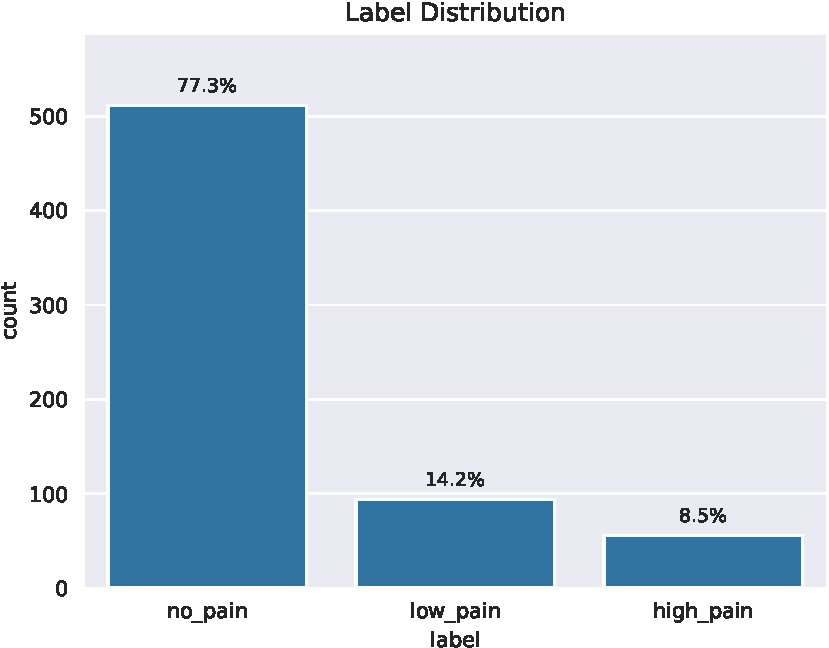
\includegraphics[width=\linewidth]{./label_distribution.pdf}
            \caption{Label distribution is strongly imbalanced toward \texttt{no\_pain}. This motivated the use of macro F1 and class balancing techniques.}
            \label{fig:label-distribution}
        \end{figure}

        \subsection*{Initial attempts}

        An initial baseline on raw sequences highlighted two issues:
        \begin{itemize}[nosep]
            \item strong bias toward \texttt{no\_pain};
            \item unstable performance on minority classes.
        \end{itemize}
        This motivated explicit temporal feature engineering and a clearer separation between static and dynamic inputs.

        \vspace{-.8em}

        \section{Method}

        \vspace{-.2em}
        \subsection*{Feature representation}
        
        Pirate traits (strings) are parsed into:
        \begin{itemize}[nosep]
            \item numeric counts of legs, hands and eyes;
            \item binary flags (peg leg, hook hand, eye patch).
        \end{itemize}
        Dynamic features:
        \begin{itemize}[nosep]
            \item surveys (ordinal, not scaled);
            \item joints (scaled continuous values).
        \end{itemize}
        Final shapes:
        \begin{itemize}[nosep]
            \item dynamic tensor: \((661,160,34)\);
            \item static vector: \((661,7)\).
        \end{itemize}

        \subsection*{Temporal feature engineering}

        To improve the quality of the temporal signal before feeding it to the model, we expand each of the 30 dynamic joints into three informative channels: (i) the raw measurement, (ii) its first temporal difference (a proxy for local velocity), and (iii) a running standard deviation computed over a nine-step window, which captures short-term instability and local noise patterns. This yields a total of 90 numerical channels per time step.

        Since it is difficult for a model to reconstruct many temporal properties (global trends, amplitude variability, and the timing of key events) from short sequences, we also provide sequence-level summary statistics for every numeric feature. These include distributional descriptors (mean, standard deviation, percentiles, and range); trend indicators (difference between the first and last samples, ordinary least squares (OLS) slope, and total variation); temporal shape cues (location of maxima and zero-crossings); and coarse time-region aggregates (statistics computed over early, mid, and late portions of the sequence). All summaries are concatenated into a fixed-size vector, standardized, and used as an additional static input. This compact representation provides the model with an overview of each joint's global behavior, reducing the burden of extracting long-term patterns from raw sequences alone.

        \vspace{-1em}

        \subsection*{Model architecture: \texttt{PainTCNBiLSTMAttn}}
        
        The model combines different architectures to effectively capture temporal patterns in the data while integrating static features. The main components are:
        \begin{enumerate}[nosep]
            \item \textbf{Embedding Layer}: each of the 4 survey inputs is passed through its own embedding layer to create dense representations.
            \item \textbf{Concatenation}: the numerical features and the survey embeddings are concatenated along the feature dimension.
            \item \textbf{Projection Layer}: the concatenated features are projected to the TCN channel dimension.
            \item \textbf{TCN Layer}: the projected features are passed through the Temporal Convolutional Network (TCN).
            \item \textbf{SE Block}: the output of the TCN is refined using a Squeeze-and-Excitation (SE) block.
            \item \textbf{BiLSTM Layer}: the refined features are processed by a Bidirectional LSTM to capture temporal dependencies.
            \item \textbf{Attention Pooling}: attention pooling is applied to obtain a fixed-size dynamic feature vector.
            \item \textbf{Static MLP}: the static features are processed through a Static Multi-Layer Perceptron (MLP).
            \item \textbf{Summary MLP}: the summary features are processed through a Summary MLP.
            \item \textbf{Gating Mechanism}: a gating mechanism modulates the dynamic feature vector based on the static and summary features.
            \item \textbf{Final Classification Head}: the concatenated dynamic, static, and summary features are passed through the final classification head to produce logits.
        \end{enumerate}
        We used a BiLSTM after TCN to capture longer-term dependencies in sequential data. The bidirectional configuration allows the LSTM to access information from both past and future contexts simultaneously. We used only one layer of LSTM because the preceding TCN already serves as a strong feature extractor. We did not use dropout in the LSTM as the preceding TCN already includes dropout for regularization.
        
        \subsection*{Training}
        
        The training phase used an extensive hyperparameter search via stratified group $5$-fold cross-validation to identify the best configuration for the \texttt{PainTCNBiLSTMAttn} model. This process was carried out in two main phases:
        \begin{enumerate}[nosep,label=\textbf{\Alph*.}]
            \item In this phase, we searched for the optimal class-2 multiplier, batch size, dropout rate, and model width by evaluating 288 configurations using 5-fold CV.
            \item The best hyperparameter combination identified in Phase A was used to train the model again using stratified group $5$-fold CV. Test-Time Augmentation (TTA)\cite{wang2018automatic} was applied during inference to improve robustness, and temperature scaling along with prior correction were employed to enhance calibration and performance on the test set.
        \end{enumerate}
        As a result, we obtained a well-calibrated and robust model capable of accurately predicting pain levels from the provided data, composed of:
        \begin{itemize}
            \item A weighted random sampler to address class imbalance during training, with a class-2 multiplier of 0.7 (balanced emphasis on class 2).
            \item A batch size of 16 to ensure stable training.
            \item A dropout rate of 0.4 to prevent overfitting.
            \item A model width of 32 for both TCN channels and LSTM hidden size, balancing model capacity and computational efficiency.
        \end{itemize}

        \vspace{-1em}
        
        \section{Experiments and Final Results}

        One of the main focuses of our experiments was to find a stable configuration that balanced performance and variance across folds. During hyperparameter tuning, we assigned different weights to the second class (\texttt{low\_pain}) to address the class imbalance. We experimented with multipliers ranging from 0.3 to 1, and the research phase concluded with an extensive grid search comprising approximately 288 configuration combinations and 5-fold cross-validation (CV), equating to 1,440 training runs ($288 \times 5 = 1.440$ training runs, $\approx 34$ hours), in order to identify the optimal class-2 multiplier, batch size, dropout rate and model width.

        To ensure robustness, we also evaluated each configuration using cross-validation, focusing on the mean and standard deviation of the macro F1 score across folds. We employed different techniques to enhance model stability, including Exponential Moving Average (EMA) of model weights during training \cite{morales2024exponential}, temperature scaling for calibration \cite{pmlr-v70-guo17a} and light Test-Time Augmentation (TTA, small noise addition and time shifts)\cite{wang2018automatic}.

        \begin{figure}[H]
            \centering
            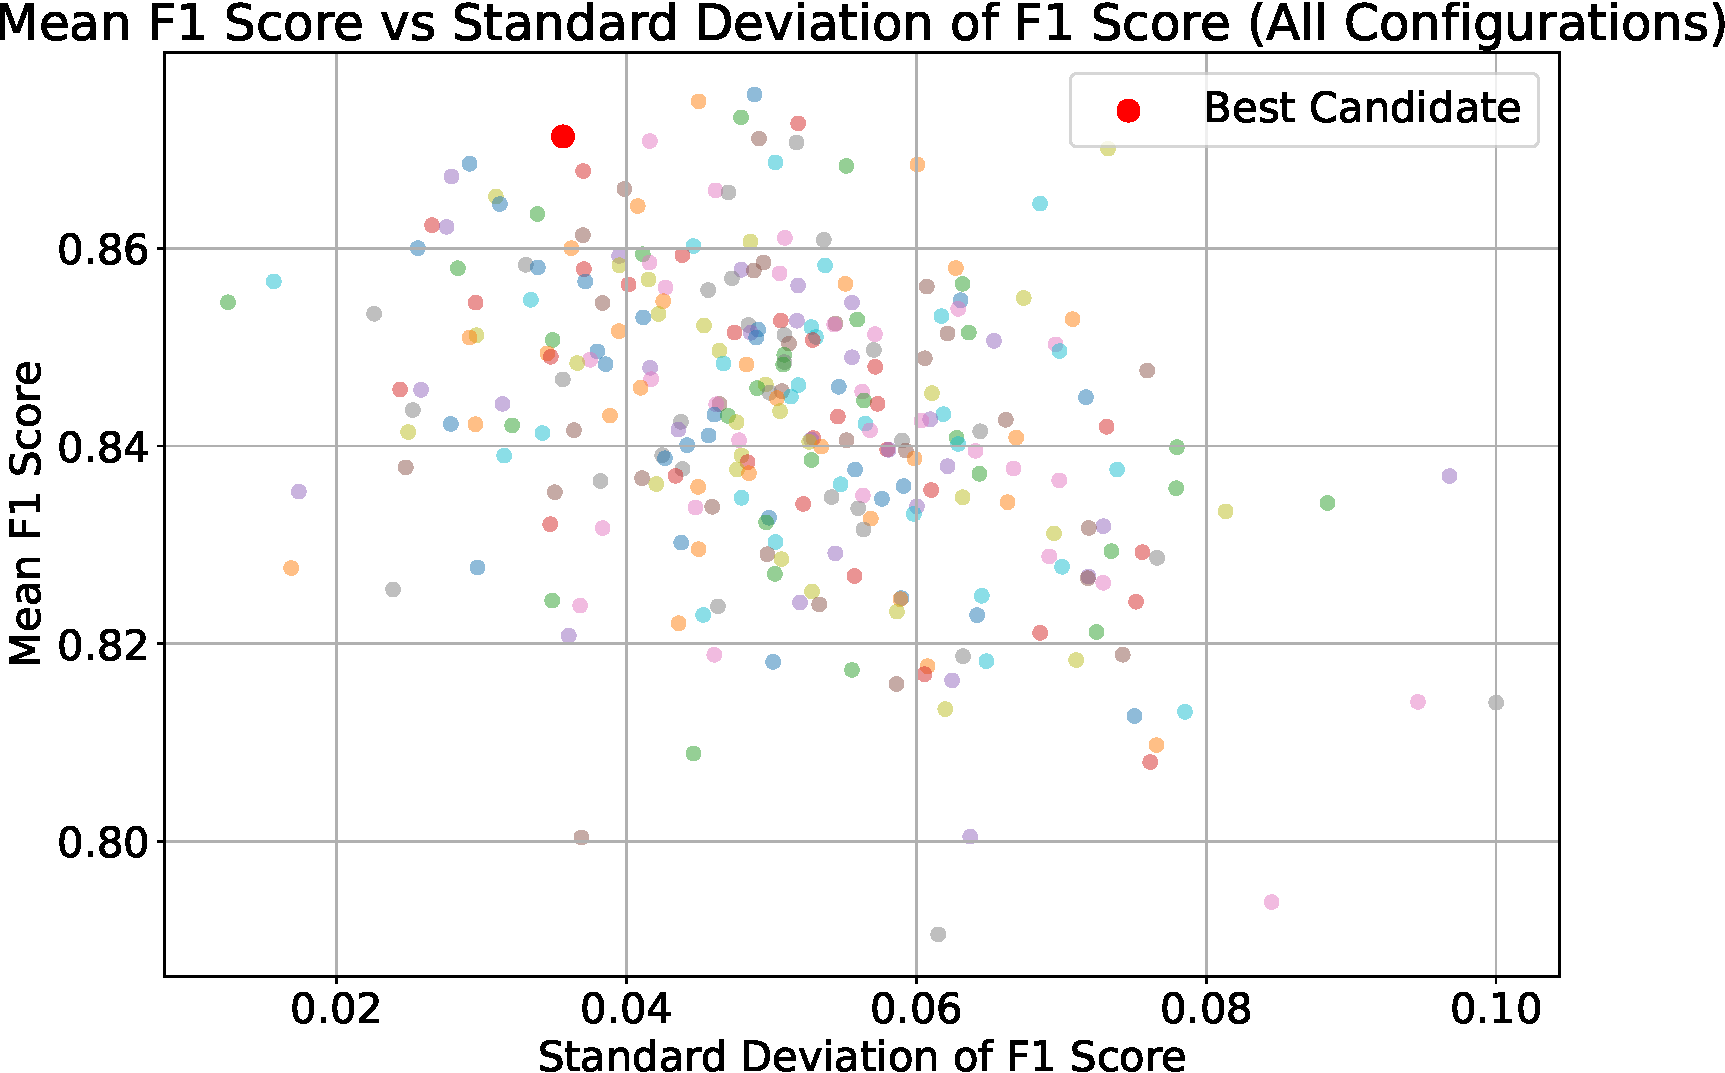
\includegraphics[width=\linewidth]{mean_f1_vs_std_f1_all_configurations.pdf}
            \caption{Although cross-validation yields a mean macro-F1 of 0.871 (std 0.036), our final \textbf{Kaggle submission scores 0.94}. This gap is expected and arises because cross-validation evaluates a model trained on only 80\% of the data and without test-time enhancements. The final model used for submission is trained on 100\% of the training set and benefits from calibration (temperature scaling, logit bias) and Test-Time Augmentation (TTA), all of which are not included in the cross-validation score. Therefore, the CV score is a conservative estimate, while the Kaggle score reflects the full model capacity and improved inference pipeline.}
            \label{fig:meanf1_vs_stdf1}
        \end{figure}

        \vspace{-1.2em}
        
        \section{Discussion and Conclusions}
        
        
        We combined temporal feature engineering and a hybrid TCN–BiLSTM–Attention architecture to address the Pirate Pain sequence classification task. Cross-validation produced a macro-F1 of 0.871 (std 0.036), confirming the stability of the selected configuration.
        
        The final model, trained on the full dataset and enhanced with calibration and Test-Time Augmentation, achieved \textbf{0.9466 macro-F1} on the test set. This improvement is expected since CV models see only 80\% of the data and exclude inference-time refinements.
        
        Given more time, potential extensions could include testing simpler baselines as additional ensemble members or trying alternative attention mechanisms.
    \end{multicols}

    \newpage

    \bibliographystyle{plain}
    \bibliography{references}
\end{document}